\documentclass[]{article}   
\usepackage{graphicx}
\usepackage{xcolor} 
\usepackage{subcaption}
\usepackage{wrapfig}
\usepackage[utf8]{inputenc}
\usepackage{amsmath}
\usepackage{float}
%\usepackage{todonotes} 
\usepackage{color}
\usepackage{epstopdf}
\usepackage{mdframed}
\usepackage[a4paper]{geometry}
\geometry{top=3cm,left=4cm, right=4cm}
\sloppy
\definecolor{lightgray}{gray}{0.5}
\setlength{\parindent}{0pt}
\renewcommand{\figurename}{Figura}
\renewcommand{\refname}{Referències}
\newcommand{\CP}[1]{\textcolor{blue}{#1}}
%SetFonts
%Title Page
\title{Robòtica industrial i de serveis. \\~\\ Projecte final \\~\\ Implementació d'estructures de control utilitzant la Robotics Toolbox. }
\author{Guillem Casado, Albert Llebaria}
\date{Gener 2019}                           
\begin{document}
\maketitle

\section{Objectius}

L'objectiu d'aquest projecte és implementar dues estructures de control per al moviment d'un robot. Aquestes són: 

\begin{itemize}
\item Controlador PD amb compensació de gravetat en l'espai d'articulacions. 
\item Control de dinàmica inversa en l'espai d'articulacions.
\end{itemize}

Per tal d'assolir-ho, s'ha de dur a terme els següents punts:

\begin{itemize}
\item Per cada estratègia de control, implementar el sistema mitjançant SIMULINK. 
\item Utilitzar la llibreria Robotic Toolbox per a la realització del projecte. 
\item Utilitzar el robot PUMA560, ja que es disposen les seves característiques (inèrcia, coriolis...) per facilitar la implementació. 
\item Proporcionar un script per configurar paràmetres com ara les constants dels controladors, configuracions inicial i final de les articulacions del robot etc.
\item Mostrar una animació del robot movent-se de posició inicial a final en cada execució del SIMULINK de cada estratègia de control. Això permet comprovar que la implementació és correcta. 
\end{itemize}

\section{Controlador PD amb compensació de gravetat en l'espai d'articulacions}

\subsection{Estudi del model teòric a implementar}
Per aquesta estructura de control, es desitja assolir una determinada configuració d'articulacions, $q_{d}$. D'aquesta manera, l'error serà $\tilde{q} = q_{d} - q$. El model del robot a controlar és $B(q)\ddot{q} + C(q, \dot{q})\dot{q} + F\dot{q} + g(q) = u$. Donada la no linealitat d'aquest, es fa ús del mètode de Lyapunov per tal de garantir que la llei de control porti al robot fins a la configuració desitjada d'una manera assimptòticament estable. La funció de Lyapunov $V(q, \dot{q})$ per aquest model és: \\

\centerline{$V(q, \dot{q}) = \frac{1}{2}\dot{q}^TB(q,\dot{q}) +  \frac{1}{2}\tilde{q}^TK_{p}\tilde{q} > 0 , \forall\dot{q},q \neq 0$ } \leavevmode \\

Si $\dot{V}(q, \dot{q}) < 0$, llavors es pot garantir l'estabilitat. La derivada de la funció de Lyapunov resulta de la següent manera: \\

\centerline{$\dot{V}(q, \dot{q})= -\dot{q}^TF(\dot{q}) + \dot{q}^T[u - g(q) - K_{p}\tilde{q}]$} \leavevmode \\

Donat que el primer terme de la derivada és sempre negatiu, una possibilitat per assegurar l'estabilitat és que el segon terme sigui zero. D'aquesta manera, es decideix que la llei de control sigui: \\

\centerline{$u = g(q) + K_{p}\tilde{q}$} \leavevmode \\

Finalment, per accelerar la convergència, s'afegeix un terme derivatiu. La llei de control final, queda doncs, expressada de la forma següent: \\

\centerline{$u = g(q) + K_{p}\tilde{q} -K_{D}\dot{q}$} \leavevmode \\

Un cop definides les equacions del sistema de control, el sistema expressat en blocs resulta com el mostrat en la figura \ref{fig:PD_block_diagram}. \\

\begin{figure}[H]
\centering
    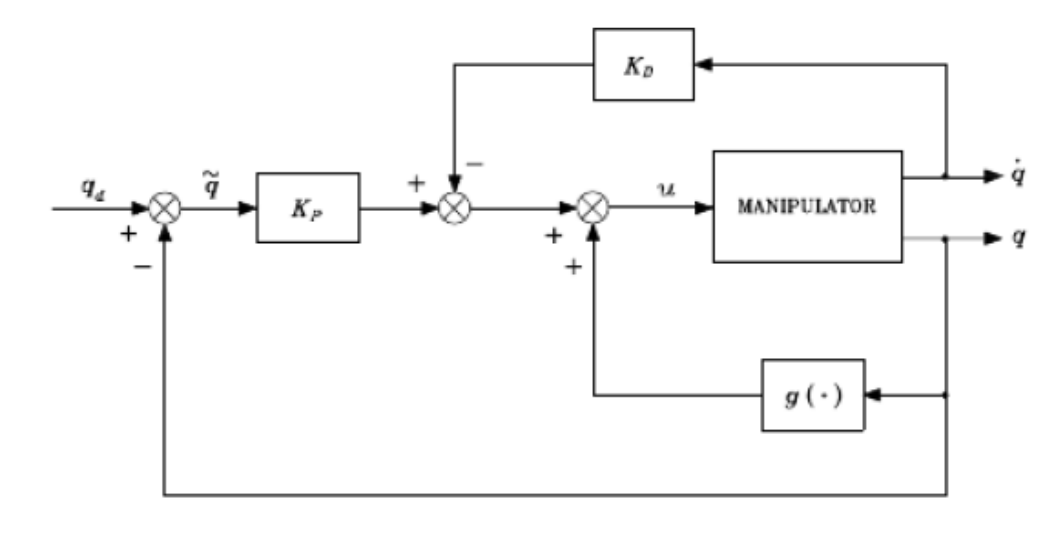
\includegraphics[width = 0.7\linewidth]{images/PD_gravity_compensation_Block_Diagram.png}
    \caption{Esquema de blocs del sistema.}
    \label{fig:PD_block_diagram}
\end{figure}

\subsection{Implementació del controlador amb Matlab}
Un cop definit el senyal de control i el diagrama de blocs, es procedeix a implementar-ho en el SIMULINK de Matlab. El resultat del diagrama de blocs es mostra en la figura \ref{fig:PD_simulink}. \\

\begin{figure}[H]
\centering
    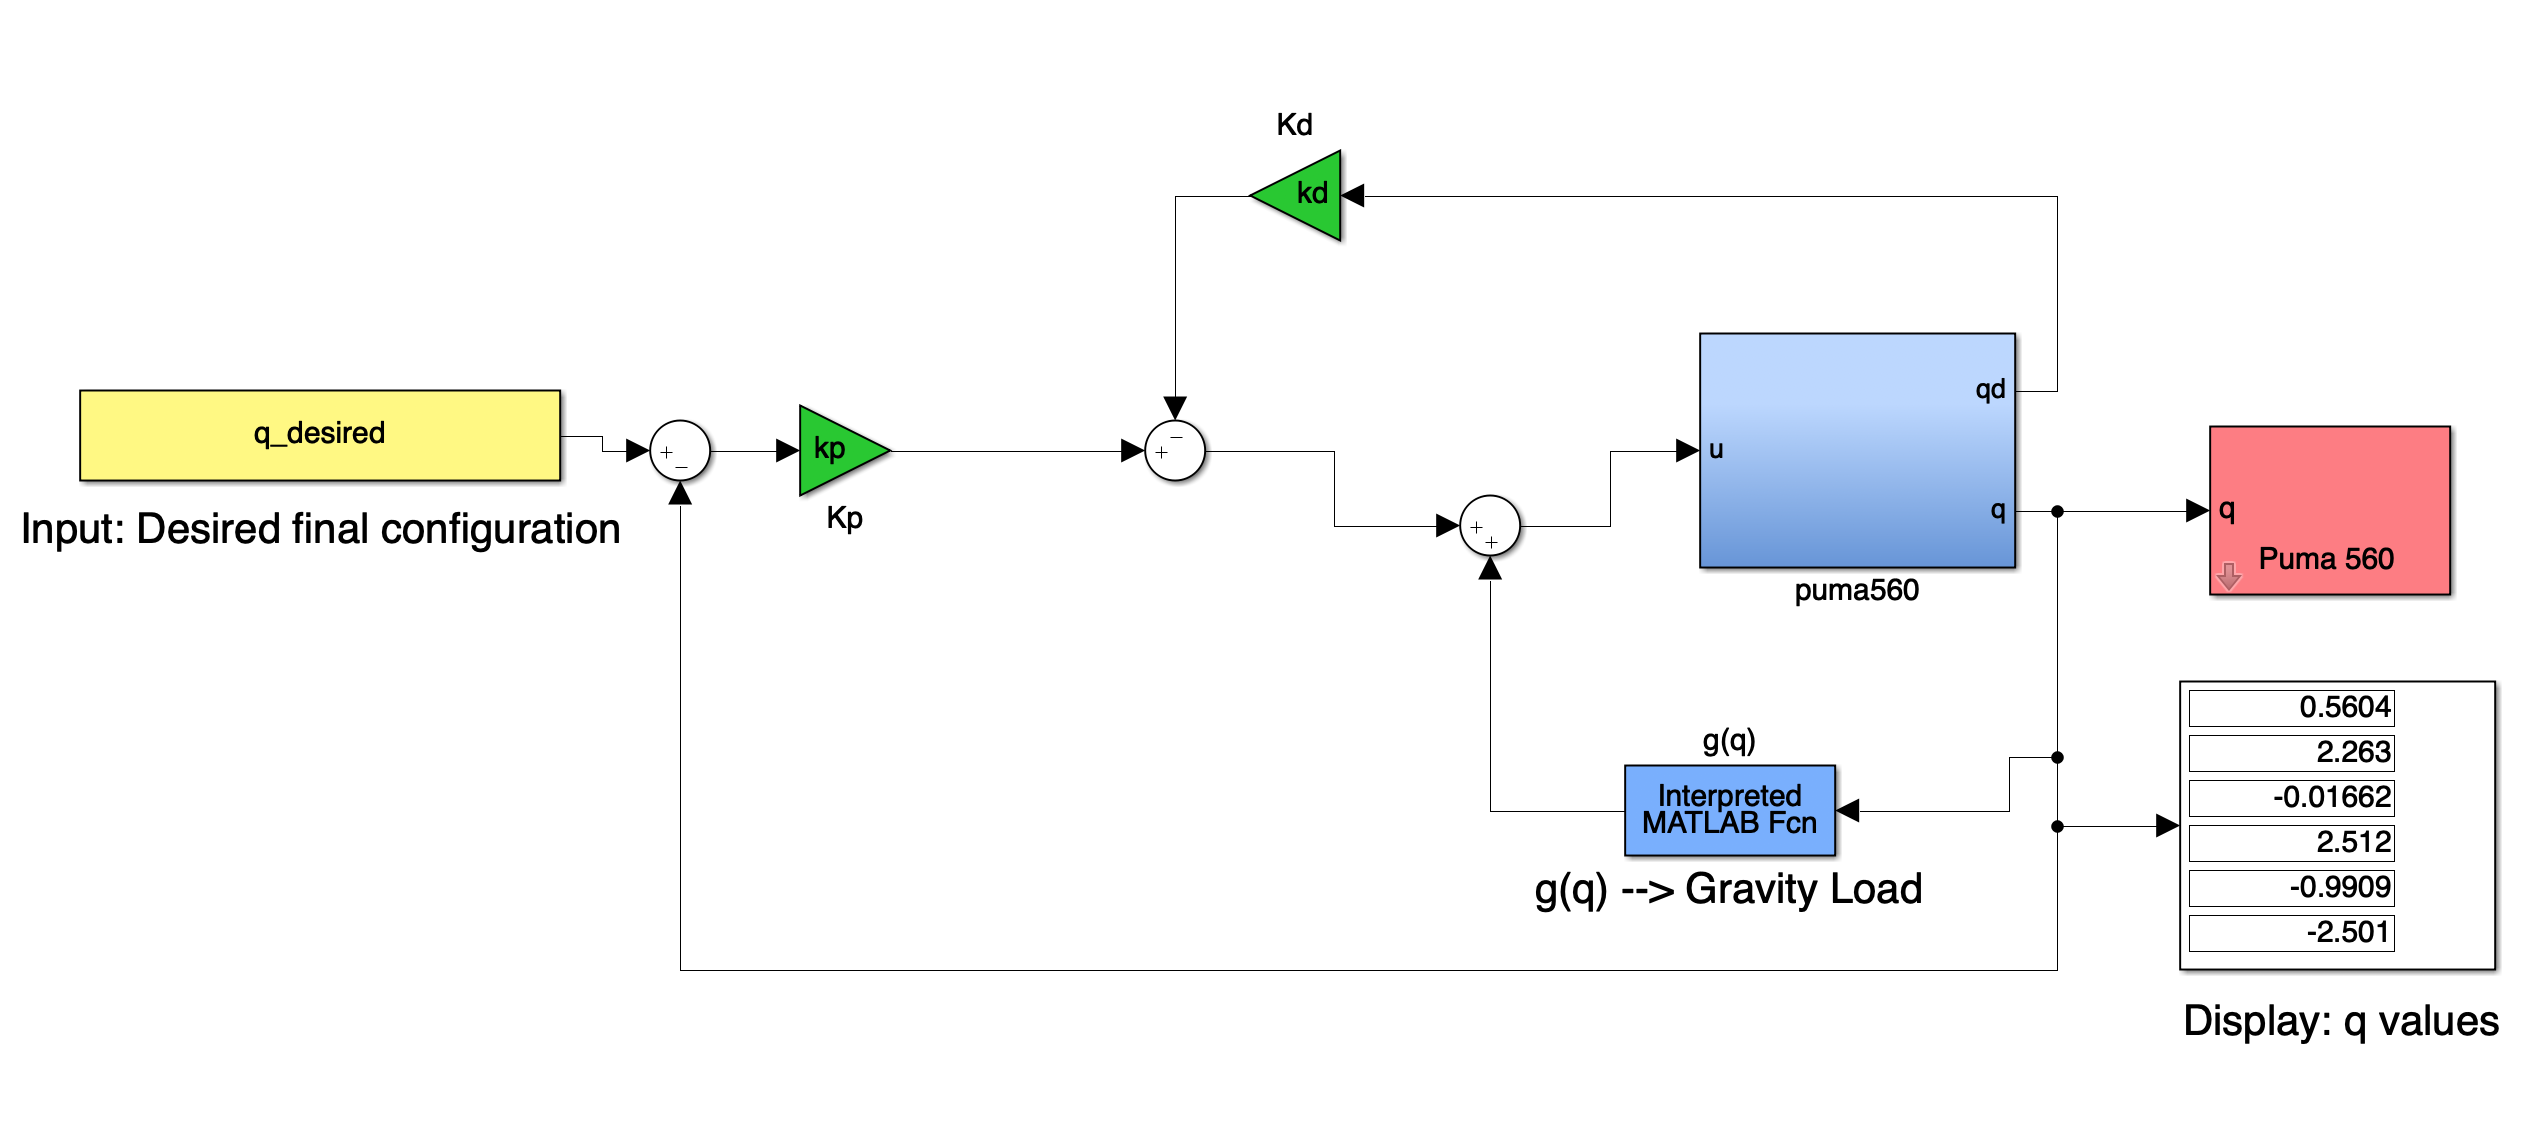
\includegraphics[width = 1\linewidth]{images/PD_gravity_compensation_Simulink.png}
    \caption{Esquema de blocs del sistema en Simulink.}
    \label{fig:PD_simulink}
\end{figure}

Els valors de $q_{d}$, $K_{p}$ i $K_{d}$ es defineixen en el script Matlab d'inicialització. El bloc $g(q)$ correspon a la compensació de gravetat donada una configuració d'articulacions. Donat que el PUMA560 ja disposa de totes les seves característiques, es pot obtenir el valor del bloc simplement amb la comanda $p560.gravload(q)$. El bloc del manipulador, rep un senyal de control que correspon al parell que han de realitzar les articulacions. La sortida d'aquest, correspon al valor de $q$ i $\dot{q}$ que s'utilitzen per al següent cicle de control. Per aconseguir-los, el que realitza el bloc manipulador és obtenir l'acceleració $\ddot{q}$ de cada articulació a partir del parell donat i, posteriorment s'integra una vegada per obtenir $\dot{q}$ i dues per trobar $q$. Cal comentar que per optimitzar l’acceleració de la convergència que proporciona el terme derivatiu, s’ha cregut convenient incorporar un saturador que evités que aquest prengués valors de magnitud massa elevada. Aquest fet podria comportar que el sistema s’inestabilitzés. Així doncs, aquest saturador ha permès augmentar el valor de la $K_{d}$ sense córrer el risc comentat. Finalment, un últim bloc es fa servir per visualitzar els resultats. Per un moviment de $q_{inicial} = [0,0,0,0,0,0]$ a $q_{d} = [\pi/4,3\pi/4,0,3\pi/4,-\pi/4,-3\pi/4]$, els resultats obtinguts són els que es mostren en la figures \ref{fig:PD_Robot_initial_q} i \ref{fig:PD_Robot_final_q}, que corresponen al robot amb la configuració inicial i final, respectivament. 

\begin{figure}[H]
\centering
    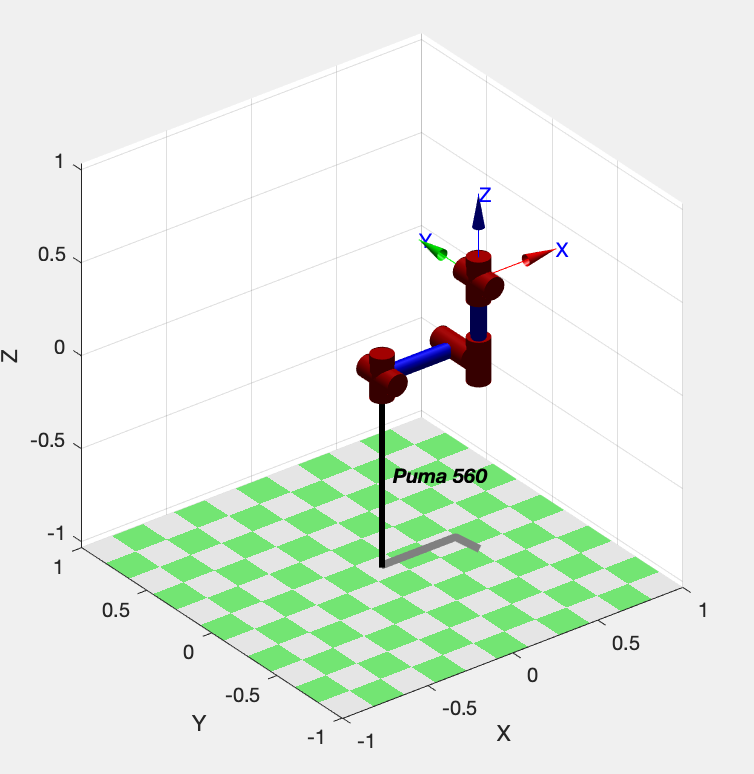
\includegraphics[width = 0.6\linewidth]{images/PD_Robot_Initial_q.png}
    \caption{Posició inicial del PUMA560.}
    \label{fig:PD_Robot_initial_q}
\end{figure}

\begin{figure}[H]
\centering
    \includegraphics[width = 0.6\linewidth]{images/PD_Robot_final_q.png}
    \caption{Posició final del PUMA560, un cop l'error ha arribat a zero.}
    \label{fig:PD_Robot_final_q}
\end{figure}

\section{Control de dinàmica inversa en l'espai d'articulacions}

\subsection{Estudi del model teòric a implementar}
Per aquesta estructura de control, s'ha de seguir una trajectòria desitjada, $q_{d}$, $\dot{q}_{d}$ i $\ddot{q_{d}}$. La dinàmica del manipulador ve descrita per la següent equació: \\

\centerline{$B(q)\ddot{q} + C(q, \dot{q})\dot{q} + F\dot{q} + g(q) = u$} \leavevmode \\

Si es defineix $n(q, \dot{q}) = C(q, \dot{q})\dot{q} + F\dot{q} + g(q)$, llavors la dinàmica del sistema queda expressada com $B(q)\ddot{q} + n(q, \dot{q}) = u$. Si ara es considera que $\ddot{q} = y$, llavors aquesta equació queda descrita en el diagrama de blocs que es mostra en la figura \ref{fig:inv_dyn_plant_bloc}. 

\begin{figure}[H]
\centering
    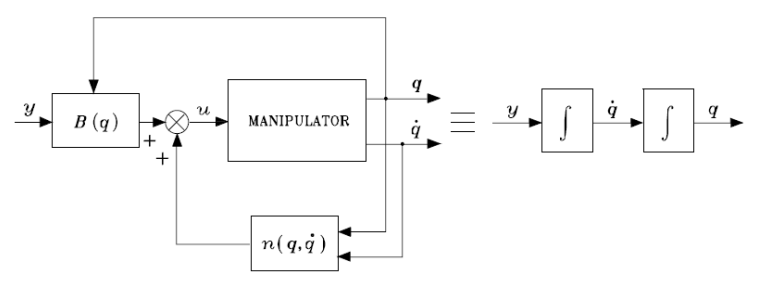
\includegraphics[width = 0.7\linewidth]{images/Inv_Dyn_Plant_Bloc.png}
    \caption{Diagrama de blocs de la dinàmica actual}.
    \label{fig:inv_dyn_plant_bloc}
\end{figure}

Tal com es pot veure, el diagrama de blocs, s'ha reduït a trobar la estabilització de la llei de control $y$. Escollint $y = -K_{p}q -K_{D}\dot{q} + r$, llavors $\ddot{q} + K_{D}\dot{q} + K_{P}q = r$. D'aquesta manera, per solucionar el problema de rastreig, $r = \ddot{q}_{d} + K_{D}\dot{q}_{d} + K_{P}q_{d}$. Així doncs, això comporta que la dinàmica de l'error vingui descrita per  $\ddot{\tilde{q}}_{d} + K_{D}\dot{\tilde{q}}_{d} + K_{P}\tilde{q}_{d} = 0$. Finalment doncs, el diagrama de blocs corresponent al sistema en llaç tancat quedaria com el que es mostra en la figura \ref{fig:inv_dyn_complete_bloc}.

\begin{figure}[H]
\centering
    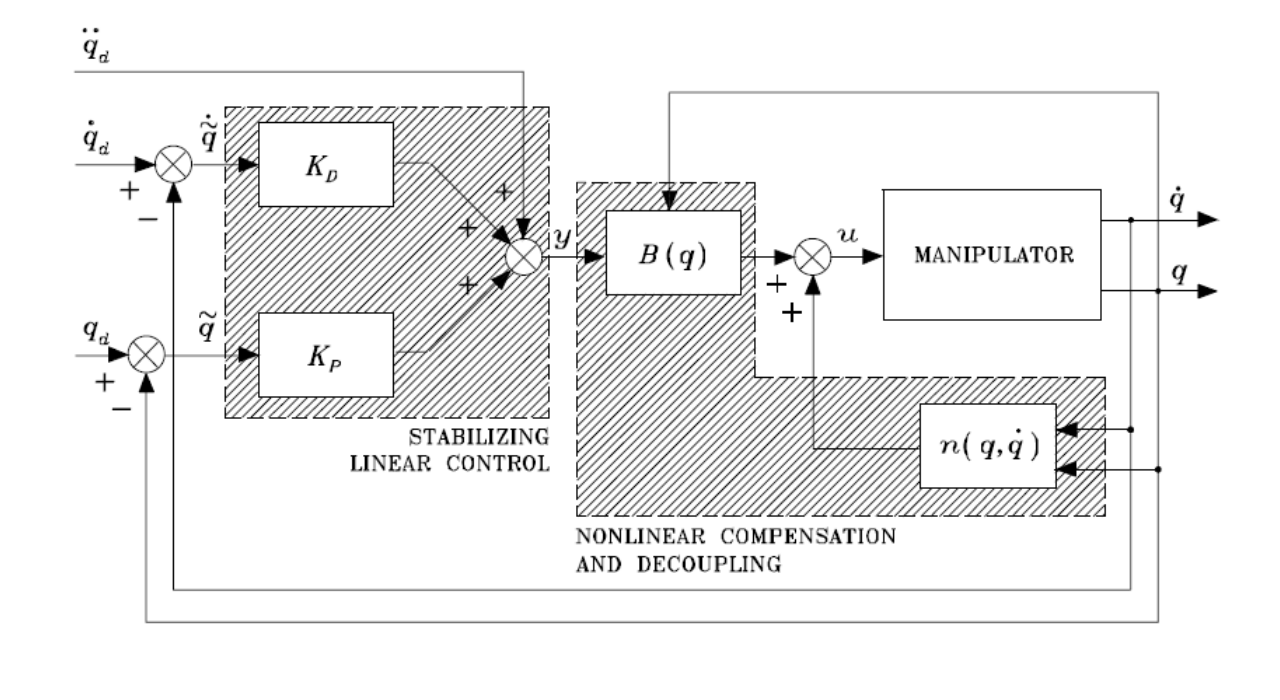
\includegraphics[width = 0.7\linewidth]{images/Inverse_Dynamics_Block_Diagram.png}
    \caption{Diagrama de blocs del sistema de control final}.
    \label{fig:inv_dyn_complete_bloc}
\end{figure}

\subsection{Implementació del controlador amb Matlab}
En primer lloc, de la mateixa manera que en el cas anterior, es programa un script de MATLAB que inicialitza els paràmetres i variables necessaris per tal de realitzar la posterior simulació. Seguidament es dissenya l'esquema de blocs que representa el sistema en el Simulink com es mostra en la figura \ref{fig:Inverse_dynamics_simulink}. 

\begin{figure}[H]
\centering
    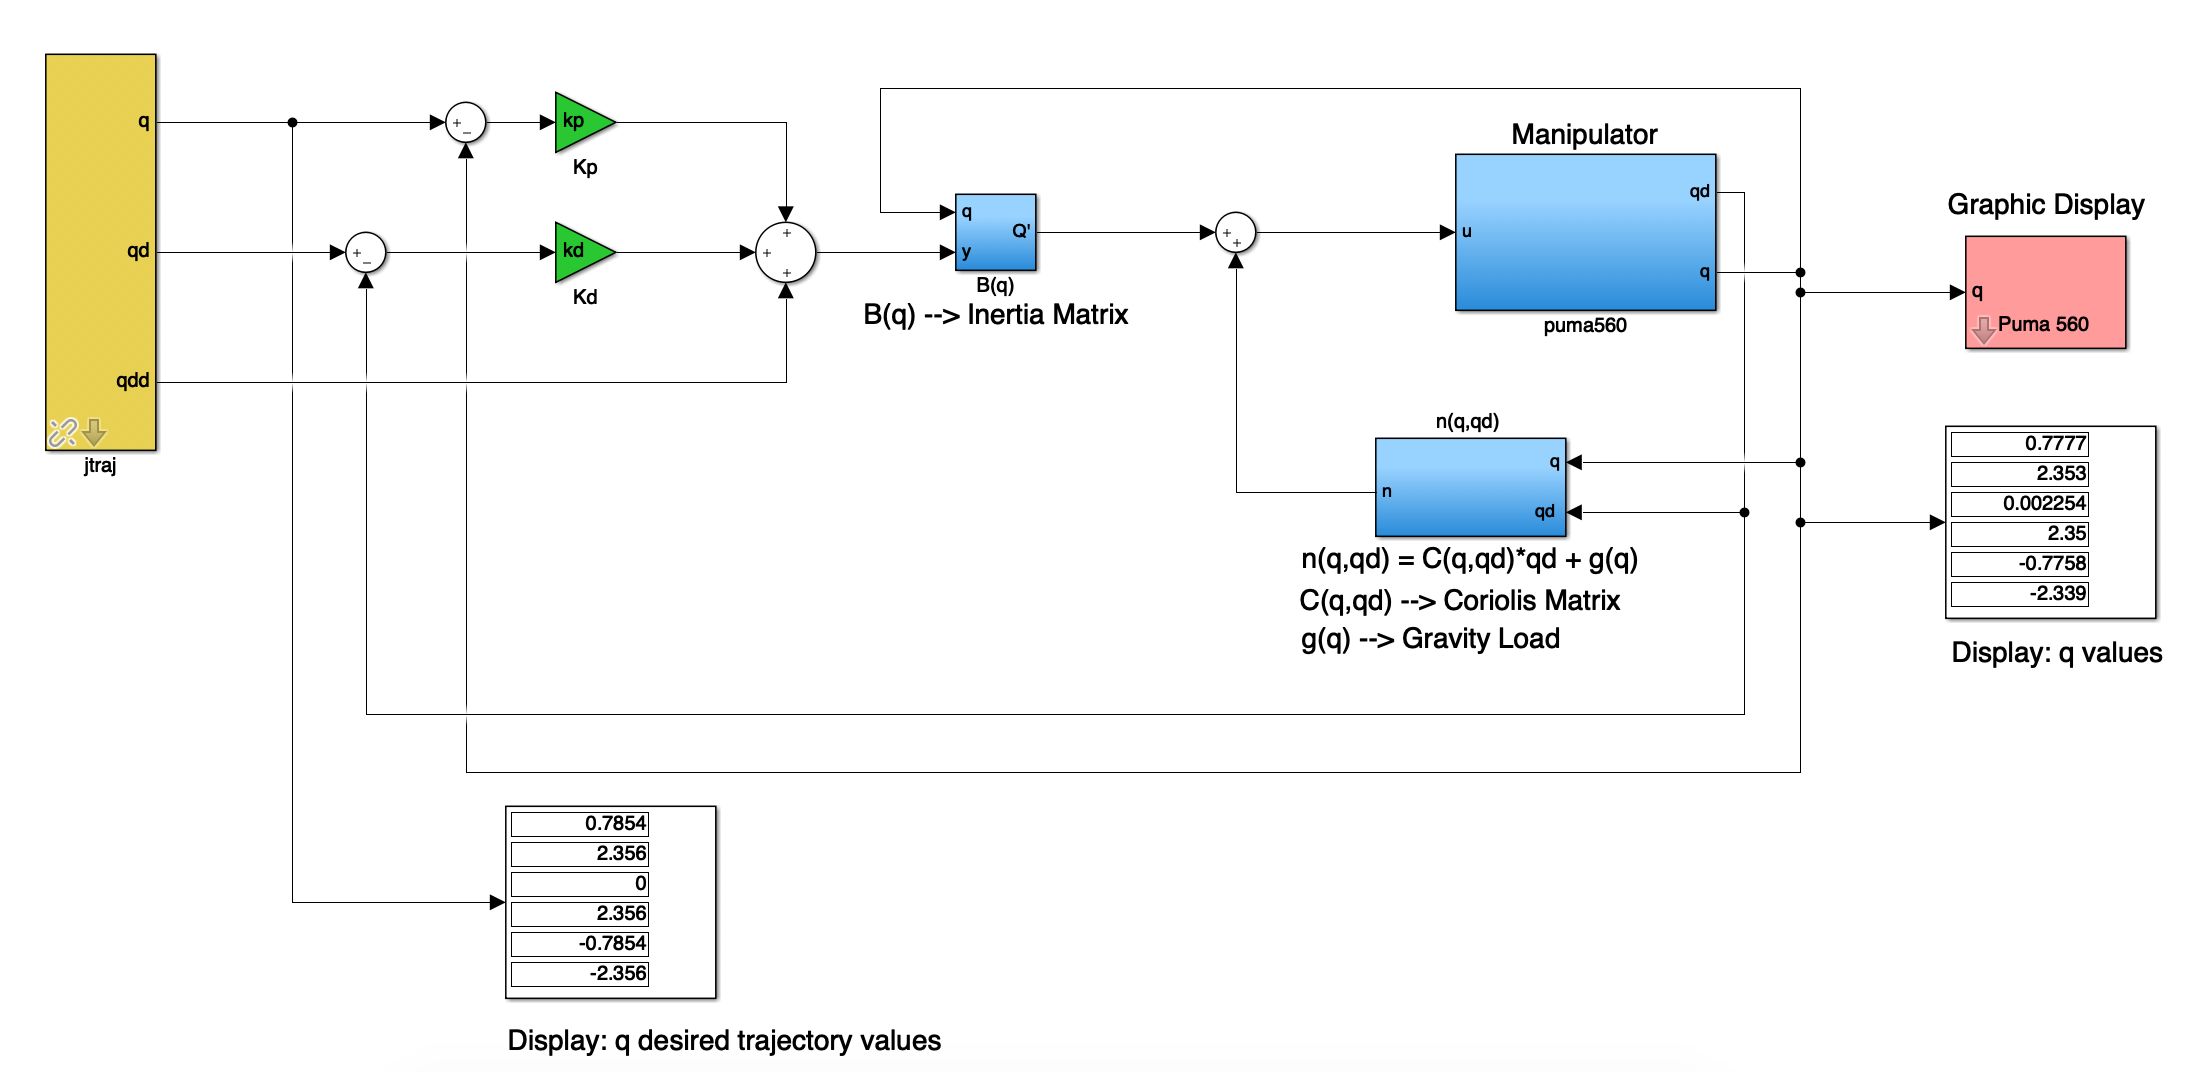
\includegraphics[width = 1\linewidth]{images/Inverse_Dynamics_Simulink.png}
    \caption{Esquema de blocs del sistema en Simulink.}
    \label{fig:Inverse_dynamics_simulink}
\end{figure}

En aquesta segona estructura de control també s'aprofiten les característiques i funcionalitats que proporciona el model del PUMA560. Concretament dins el bloc $n(q,\dot{q})$ es criden funcions com $p560.gravload(q)$ que, com s'ha comentat, proporciona la càrrega que provoca la gravetat per a una configuració determinada i $p560.coriolis(q,\dot{q})$ que retorna la matriu de forces centrífugues i de Coriolis del sistema. En relació al bloc $B(q)$, s'ha emprat la funció $p560.inertia(q)$ que proporciona la matriu d'inèrcies del sistema. El bloc que representa el manipulador està definit de la mateixa manera que en el cas anterior.\\

Finalment, per tal de aportar el senyal d'entrada s'ha optat per un bloc generador de trajectòria. Aquest bloc rep com a paràmetres la posició inicial i final així com el temps de duració màxim de la trajectòria i l'interval de temps al que ha d'anar generant les dades.\\

A continuació es mostren les figures \ref{fig:Inverse_dynamics_initial} i \ref{fig:Inverse_dynamics_final} que representen la configuració inicial del robot ($q_{inicial} = [0,0,0,0,0,0]$) i a la que arriba aquest un com realitzada tota la trajectòria ($q_{d} =[pi/4,3*pi/4,0,3*pi/4,-pi/4,-3*pi/4]$).

\begin{figure}[H]
\centering
    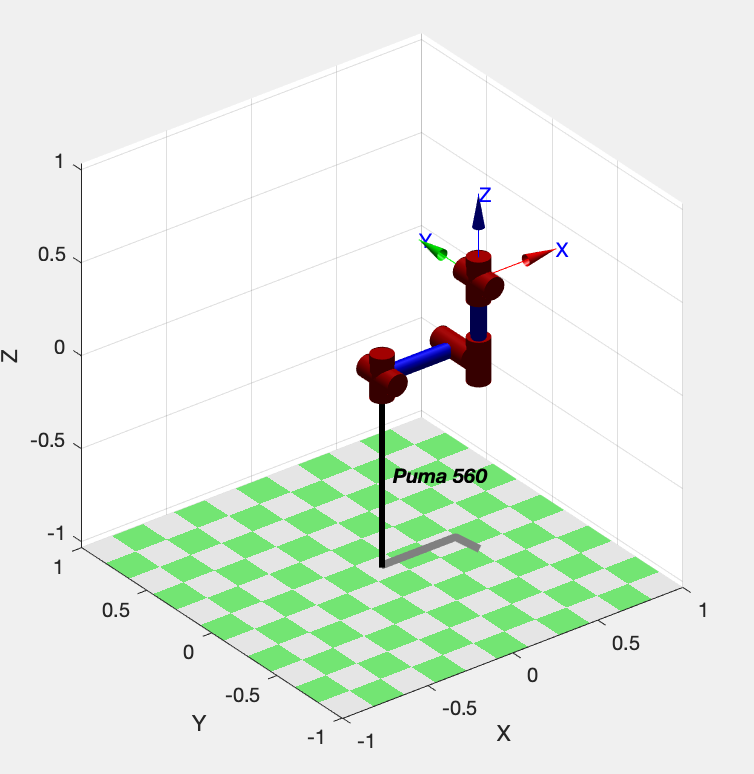
\includegraphics[width = 0.6\linewidth]{images/PD_Robot_Initial_q.png}
    \caption{Posició inicial del PUMA560.}
    \label{fig:Inverse_dynamics_initial}
\end{figure}

\begin{figure}[H]
\centering
    \includegraphics[width = 0.6\linewidth]{images/PD_Robot_final_q.png}
    \caption{Posició final del PUMA560, un cop realitzada tota la trajectòria.}
    \label{fig:Inverse_dynamics_final}
\end{figure}

Com es pot comprovar, la configuració inicial i final del robot es la mateixa que en el primer control. Donat que en aquest segon cas, també s'assoleix aquesta última posició i s'ha comprovat com es desenvolupa correctament el seguiment de la trajectòria, es dona per vàlid el funcionament i resultats de la implementació d'aquesta segona estructura de control.


\begin{thebibliography}{5}
\bibitem{latexcompanion}
Alireza. Izadbakhsh. \textit{Closed-Form Dynamic Model of  PUMA 560 Robot Arm}.
Garmsar. Iran. Febrer 2009.

\bibitem{latexcompanion}
Atta Oveisi, Miad Jarrahi, Mohammad Gudarzi and Mohammad Mahdi Mohammadi  \textit{Genetic Algorithm and Adaptive Model Reference Controller in Tracking Problem of PUMA 560 Arm Robot}.
Teheran. Iran. Febrer 2013.

\bibitem{latexcompanion}
B.Morales and R.Carelli. \textit{Robot control with inverse dynamics and non-linear gains}.
San Juan. Argentina.

\bibitem{latexcompanion}
Reham H. Mohammed, Fahmy Bendary and Kamel Elserafi. \textit{Trajectory Tracking Control for Robot Manipulator using Fractional Order-Fuzzy-PID Controller}.
Egipte. Gener 2019.

\bibitem{knuthwebsite}
Peter Corke: Robotics Toolbox for MATLAB,
\\\texttt{http://petercorke.com/wordpress/toolboxes/robotics-toolbox}
\end{thebibliography}


\end{document}